%!TEX root = ../rapport.tex
%!TEX encoding = UTF-8 Unicode

% Chapitres "Introduction"

% modifié par Francis Valois, Université Laval
% 31/01/2011 - version 1.0 - Création du document

\chapter{Modélisation de l'alimentation électronique}
\section{Fonctionnement d'un redresseur monophasé simple alternance}
Le redresseur monophasé simple alternance est composé d'une source de courant alternatif, d'un interrupteur de type IGBT et d'une charge quelquonque tel que présenté à la figure \ref{fig:RedresseurMonophaseSimpleAlternanceIGBT}. Pour les besoin de l'exemple, une charge $RL$ théorique sera utilisée où la résistance se nomme $R$ et l'inductance $L$. De plus, l'on suppose que l'interrupteur IGBT entre en conduction lorsqu'un échelon de tension unitaire est appliqué à la grille de celui-ci. Finalement, en suposant des modèles sans perte, l'équation de circuit se résume à celle présentée à l'équation \ref{eq:RLSimple}. À noter que l'échelon unitaire est défini comme: $u(t<0) = 0, u(t\geq 0) = 1)$.

\begin{figure}[htb!]
	\begin{center}  
		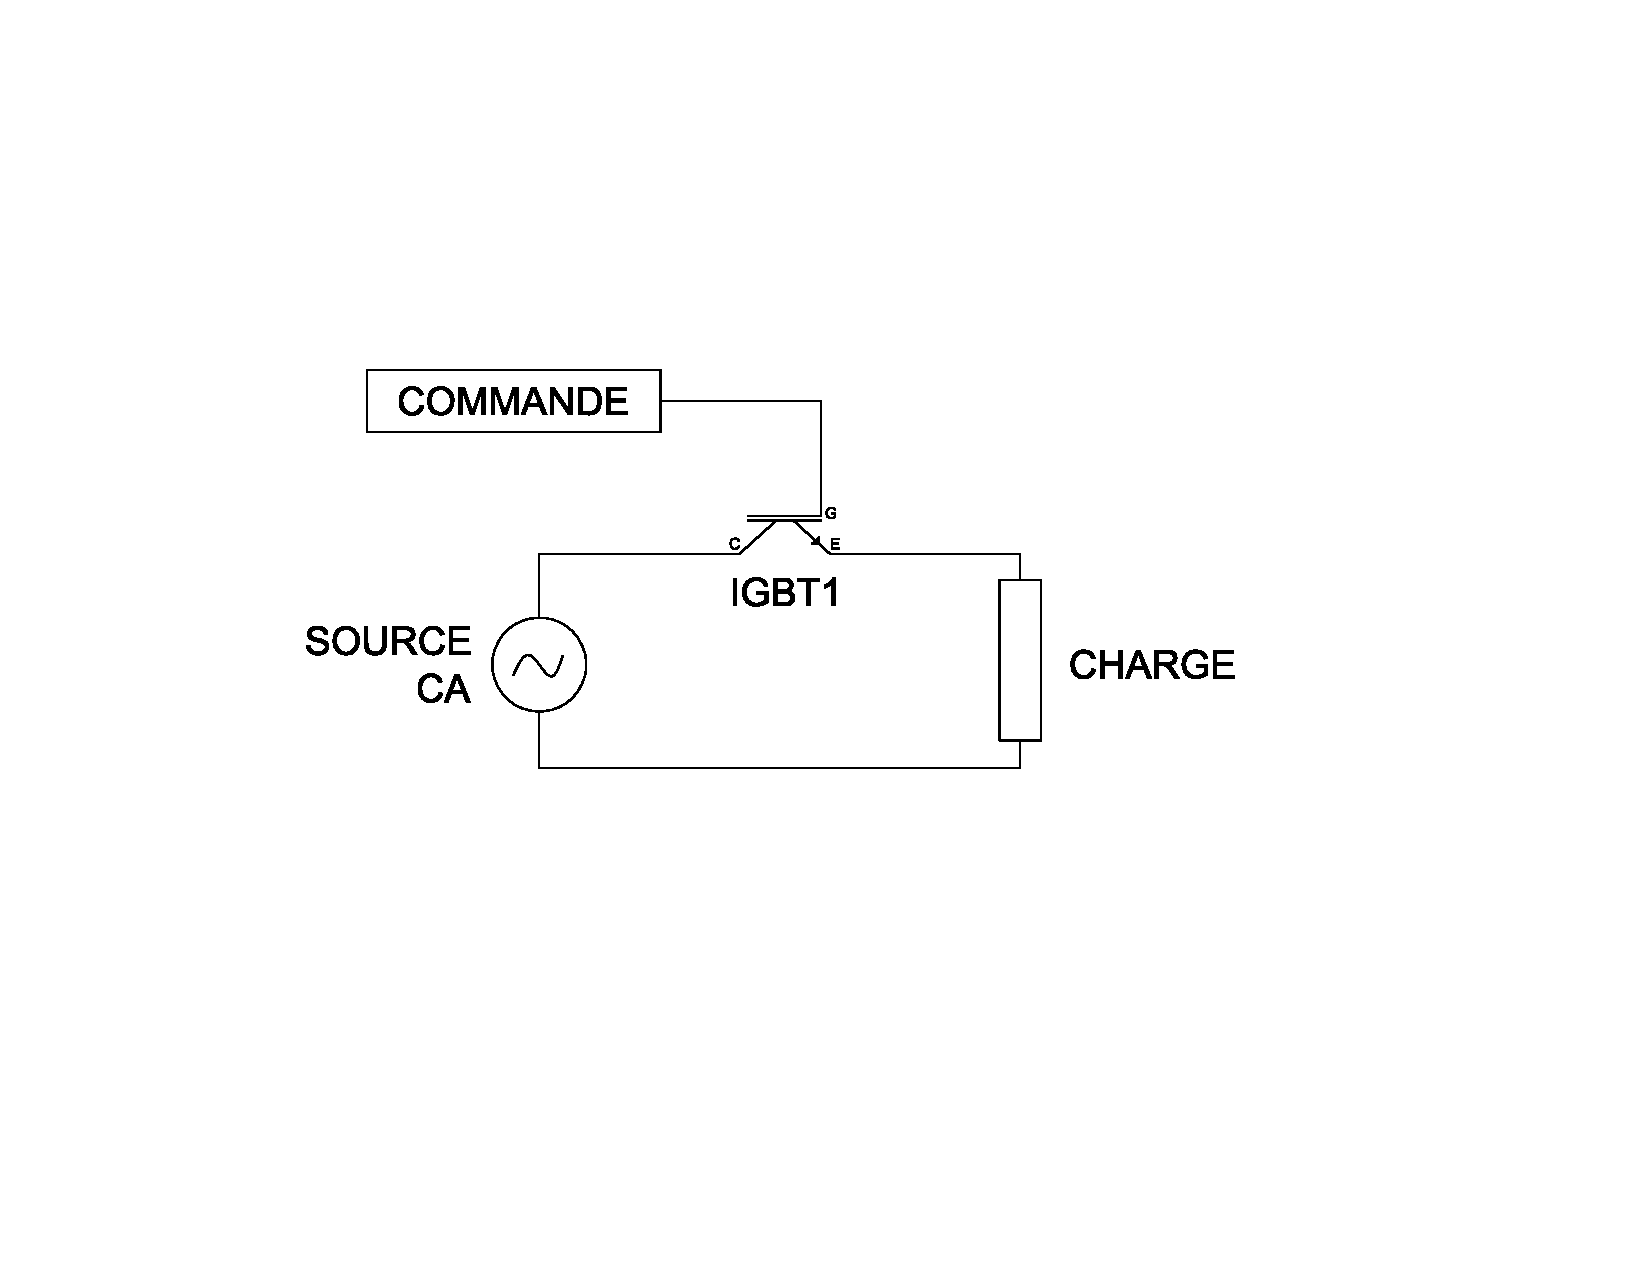
\includegraphics[width=0.7\textwidth]{Circuit/RedresseurMonophaseSimpleAlternanceIGBT}
		\caption{Circuit redresseur monophasé simple alternance avec IGBT et charge quelquonque}
		\label{fig:RedresseurMonophaseSimpleAlternanceIGBT}
	\end{center}   
\end{figure}


\begin{equation}
\label{eq:RLSimple}
v(t) = R i(t) + L \frac{d i(t)}{dt}
\end{equation}

Si l'on suppose la conduction continue de l'IGBT, il est possible d'exprimer le courant dans la charge en fonction de la tension de la source CA:

\begin{eqnarray}
V_{in}(t) &=& E_m\sin{\omega_0 t} \\
|Z| &=& \sqrt{R^2 + (\omega_0 L)^2} \\
\tau &=& \frac{L}{R}\\
\phi &=& \mbox{atan}(\omega_0 \tau) = \mbox{atan}(\omega_0 \frac{L}{R}) \\
\label{eq:solutionRLSimple} i(t) &=& \frac{E_m\sin{\phi}}{|Z|}\mbox{e}^{\frac{-t}{\tau}} + \frac{E_m\sin{(\omega_0 t + \phi})}{|Z|}\\
i(t=0) &=& i_0\\
i(t) &=& i_0  + \frac{E_m\sin{\phi}}{|Z|}\mbox{e}^{\frac{-t}{\tau}} + \frac{E_m\sin{(\omega_0 t + \phi})}{|Z|} \\
\end{eqnarray}

L'équation \ref{eq:solutionRLSimple} est la solution de l'équation différentielle \ref{eq:RLSimple} d'un circuit RL avec la partie de gauche qui est la composante transitoire et la partie de droite qui est la composante permanente. 

\paragraph{}
La fonction principale d'un redresseur est de produire une tension et un courant qui sont strictement positif. Dans le cas du redresseur simple alternance, seulement la partie positive de la source de courant alternative est envoyé à la charge et la partie négative est bloquée par l'IGBT. De plus, gràce à la commande de l'IGBT, il est possible de contrôler le temps de conduction de la partie positive du signal.

Ainsi, si l'on définit le temps total d'une période du signal par $T$, le temps de début de conduction de l'IGBT par $t_{on}$ et le temps de début de blocage par $t_{off}$, il est possible de définir le rapport de modulation $m = 2\cdot \frac{t_{off}-t_{on}}{T}$. Supposons un rapport de modulation $m_x$, il est possible, si l'on considère le courant initial nul et des temps de commutation instantannés, d'exprimer le courant dans la charge RL pour une période étant égale à $T$.

Les figures \ref{fig:RedresseurMonophaseSimpleAlternanceIGBTCourbes50} et \ref{fig:RedresseurMonophaseSimpleAlternanceIGBTCourbes100} présentent la tension et le courant dans la charge avec 2 différents niveaux de modulation. 

\begin{figure}
        \centering       
        \begin{subfigure}[Courant dans la charge en fonction de la tension dans la charge pour une modulation de 50\% avec un temps de début de conduction de 10\%]{
         		\label{fig:RedresseurMonophaseSimpleAlternanceIGBTCourbes50}
                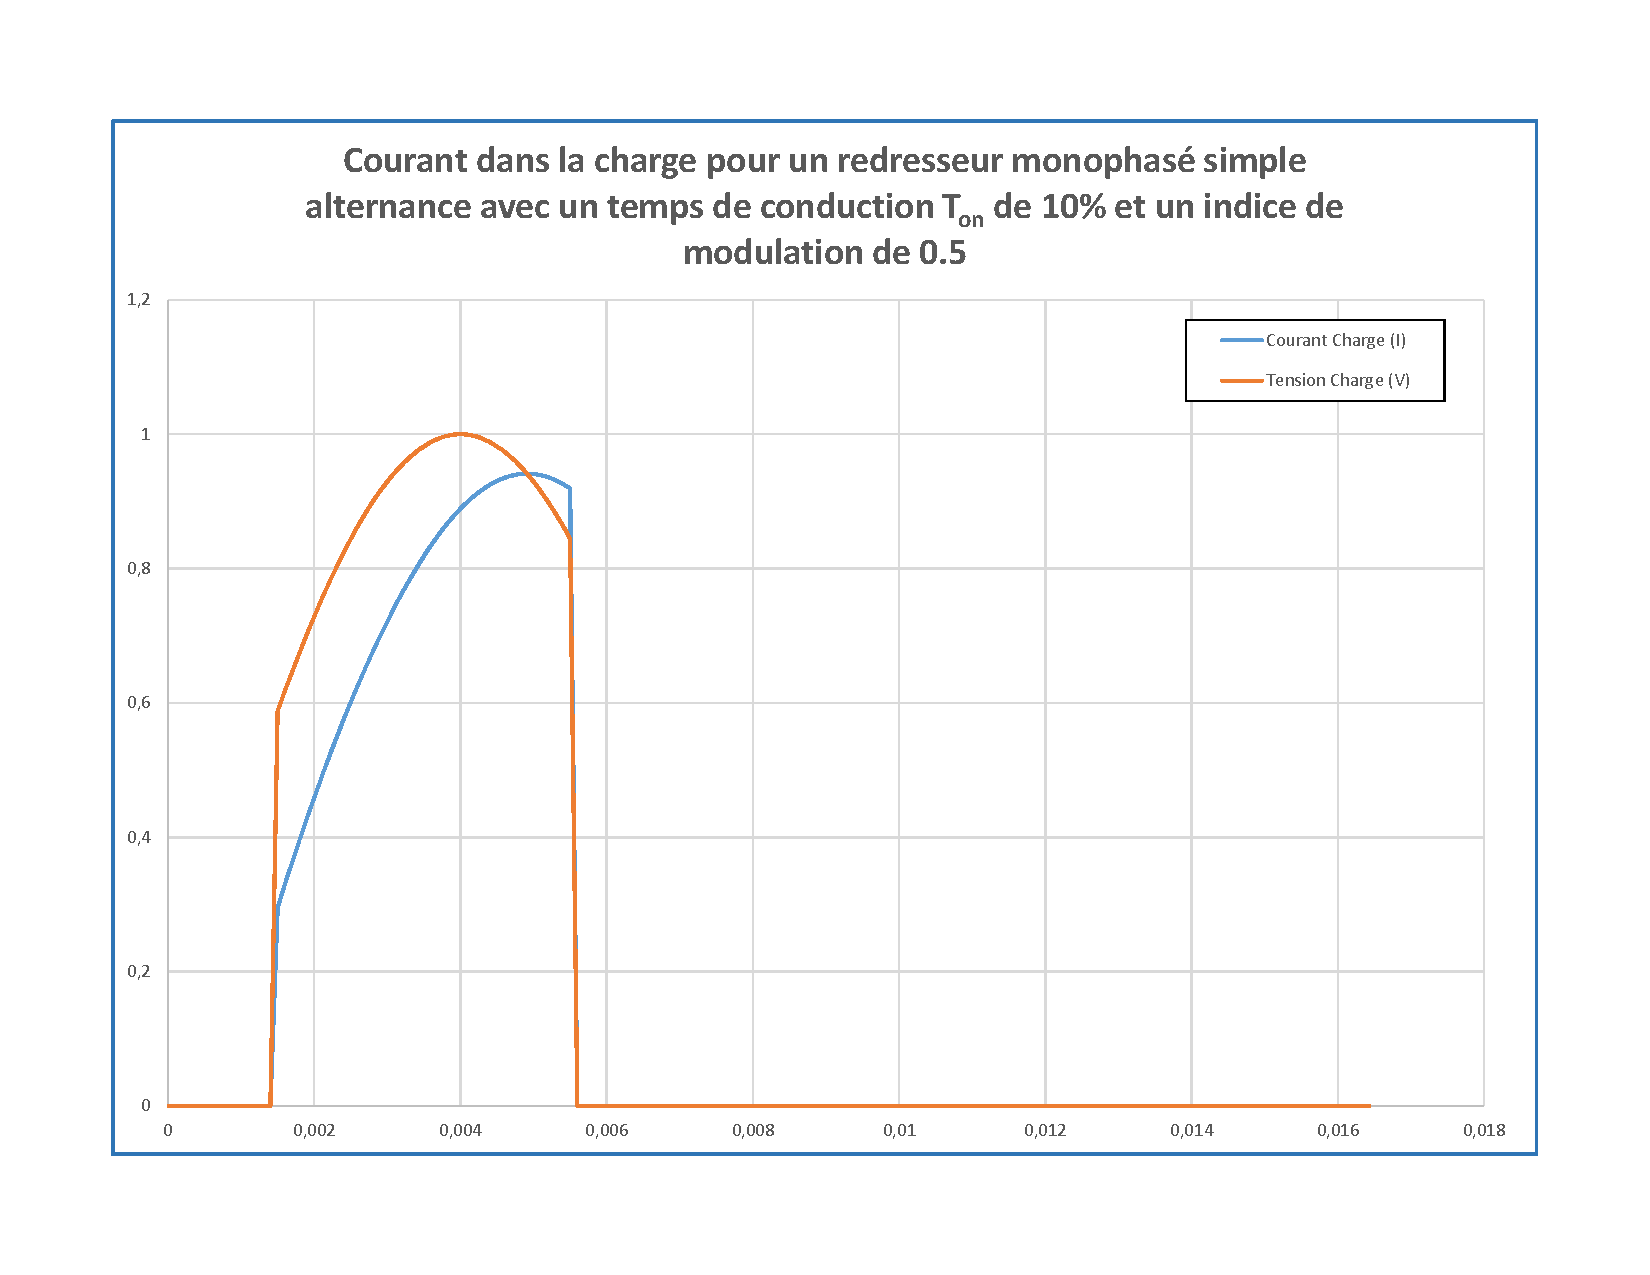
\includegraphics[width=0.68\textwidth]{Graphs/RedresseurMonophaseSimpleAlternance50}}
        \end{subfigure}        
        \begin{subfigure}[Courant dans la charge en fonction de la tension dans la charge pour une modulation de 100\% avec un temps de début de conduction de 0\%]{
         		\label{fig:RedresseurMonophaseSimpleAlternanceIGBTCourbes100}
                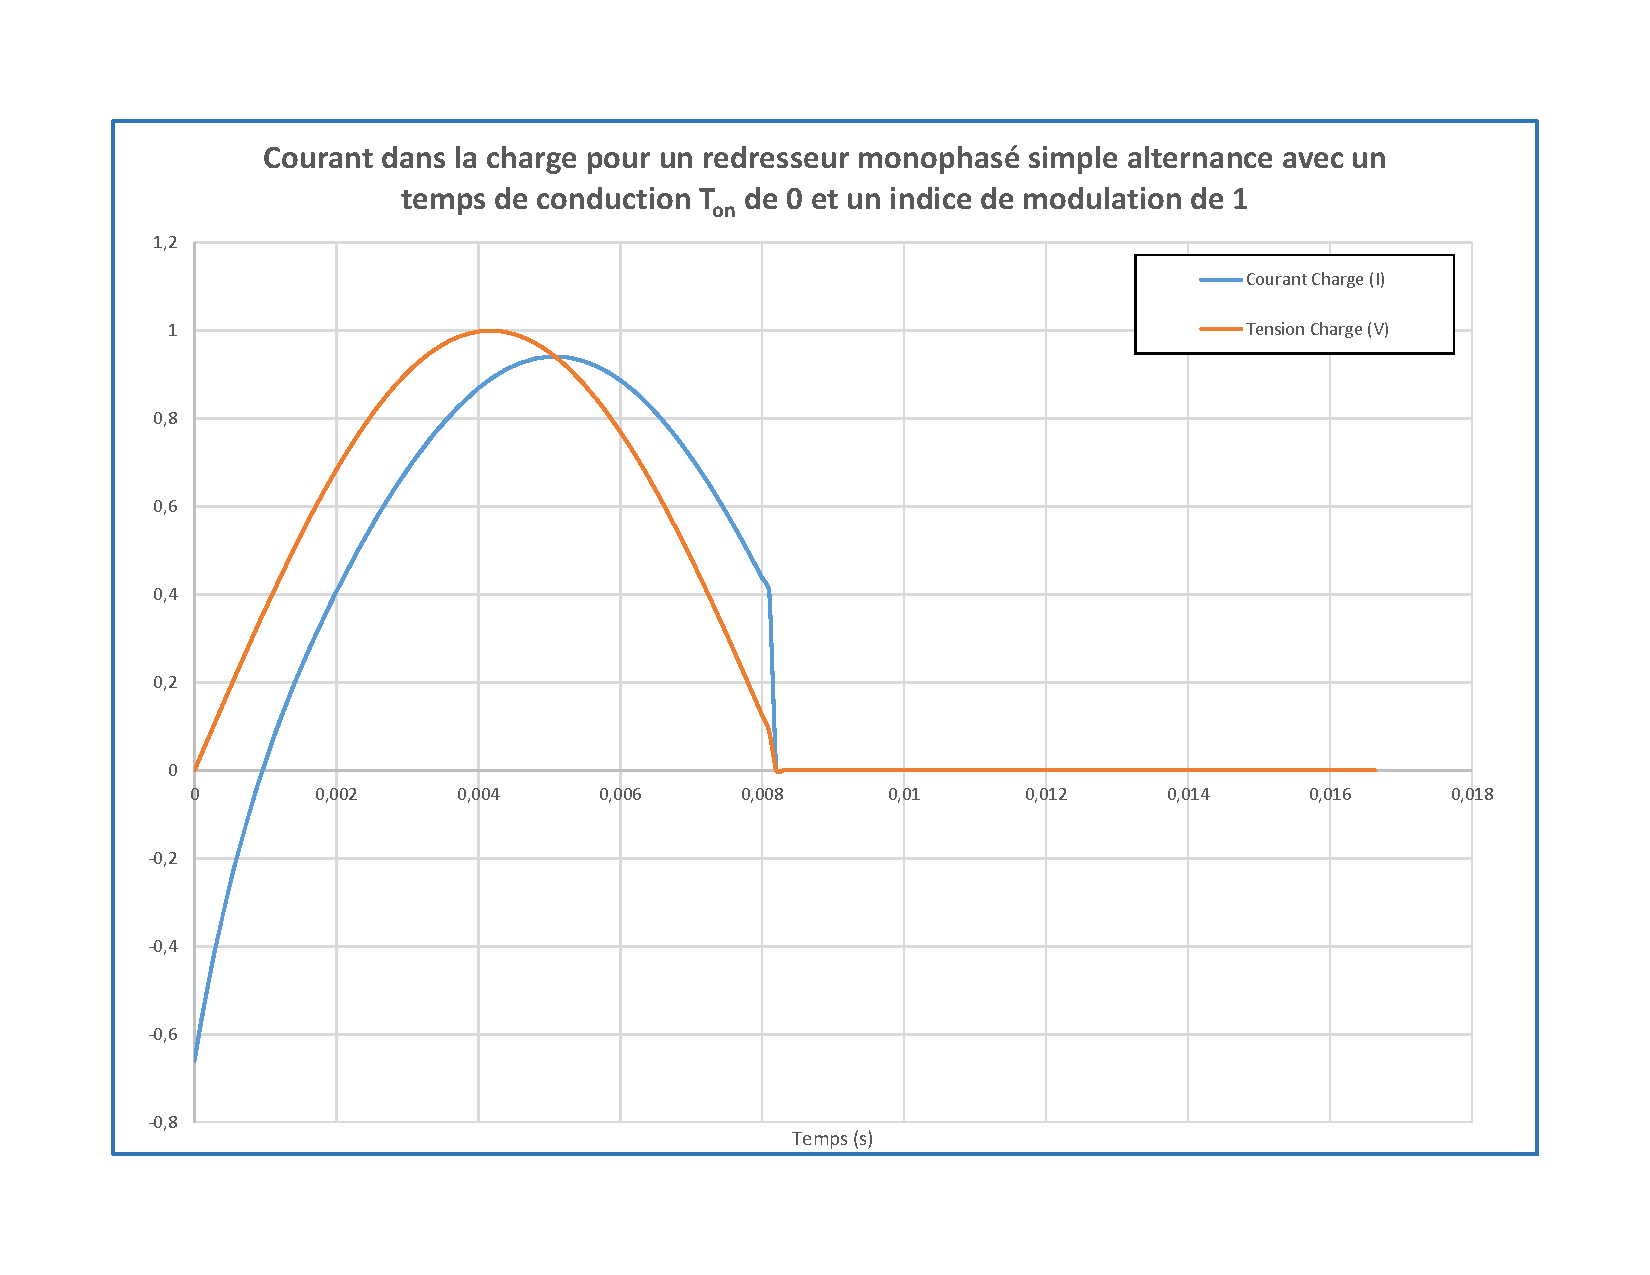
\includegraphics[width=0.68\textwidth]{Graphs/RedresseurMonophaseSimpleAlternance100}}
        \end{subfigure}
        \caption{Forme du courant et de la tension dans la charge pour 2 différents niveaux de modulation du redresseur monophasé à simple alternance}\label{fig:RedresseurMonophaseSimpleAlternanceIGBTCourbes}
\end{figure}

Comme la forme d'onde de tension et de courant dépend entièrement du niveau de modulation choisi, il est intéressant d'obtenir les valeurs de tension et de courant moyen en fonction des paramètres de modulation. La valeur moyenne du courant sur une période se calcule comme suit :

\begin{eqnarray}
I_{moy} &=& \frac{1}{T}\int_{t_{on}}^{t_{off}} i(t) dt \\
I_{moy} &=& \frac{1}{T}\int_{t_{on}}^{t_{off}} \left( \frac{E_m\sin{\phi}}{|Z|}\mbox{e}^{\frac{-t}{\tau}} + \frac{E_m\sin{(\omega_0 t + \phi})}{|Z|}\right) dt \\
I_{moy} &=& \frac{E_m}{T} \left( \frac{-\mbox{e}^{-\frac{t_{off}}{\tau}}\sin{(\phi)}\omega_0 \tau + \mbox{e}^{-\frac{t_{on}}{\tau}} + \cos{(\omega_0 t_{on} + \phi)}-\cos{(\omega_0 t_{off} + \phi)}}{|Z|\omega_0} \right)
\end{eqnarray}

Par la suite, la valeur moyenne de la tension se calcule comme suit : 
\begin{eqnarray}
V_{moy} &=& \frac{1}{T}\int_{t_{on}}^{t_{off}} V_{in}(t) dt \\
V_{moy} &=& \frac{1}{T}\int_{t_{on}}^{t_{off}} (E_m \sin{\omega_0 t}) dt \\
V_{moy} &=& \frac{E_m}{T} \left( \frac{\cos{(\omega_0 t_{on})} - \cos{(\omega_0 t_{off})}}{\omega_0} \right)
\end{eqnarray}

\section{Fonctionnement d'un redresseur monophasé double alternance}
Le schéma du redresseur monophasé double alternance est présenté à la figure \ref{fig:RedresseurMonophaseDoubleAlternanceIGBT}. Un redresseur double alternance est composé de 2 IGBT et d'une charge quelquonque. Le principal avantage par rapport au redresseur simple alternance est la possibilité d'inverser la partie négative du signal alternatif. En effet, lors de la partie positive de l'onde, les IGBT 1 et 3 vont s'activer ce qui va permettre d'alimenter la charge avec une tension positive et lors de la partie négative de l'onde, les IGBT 2 et 4 vont conduire et ainsi alimenter la charge avec une tension redressée. 

\begin{figure}[htb!]
  \begin{center}  
    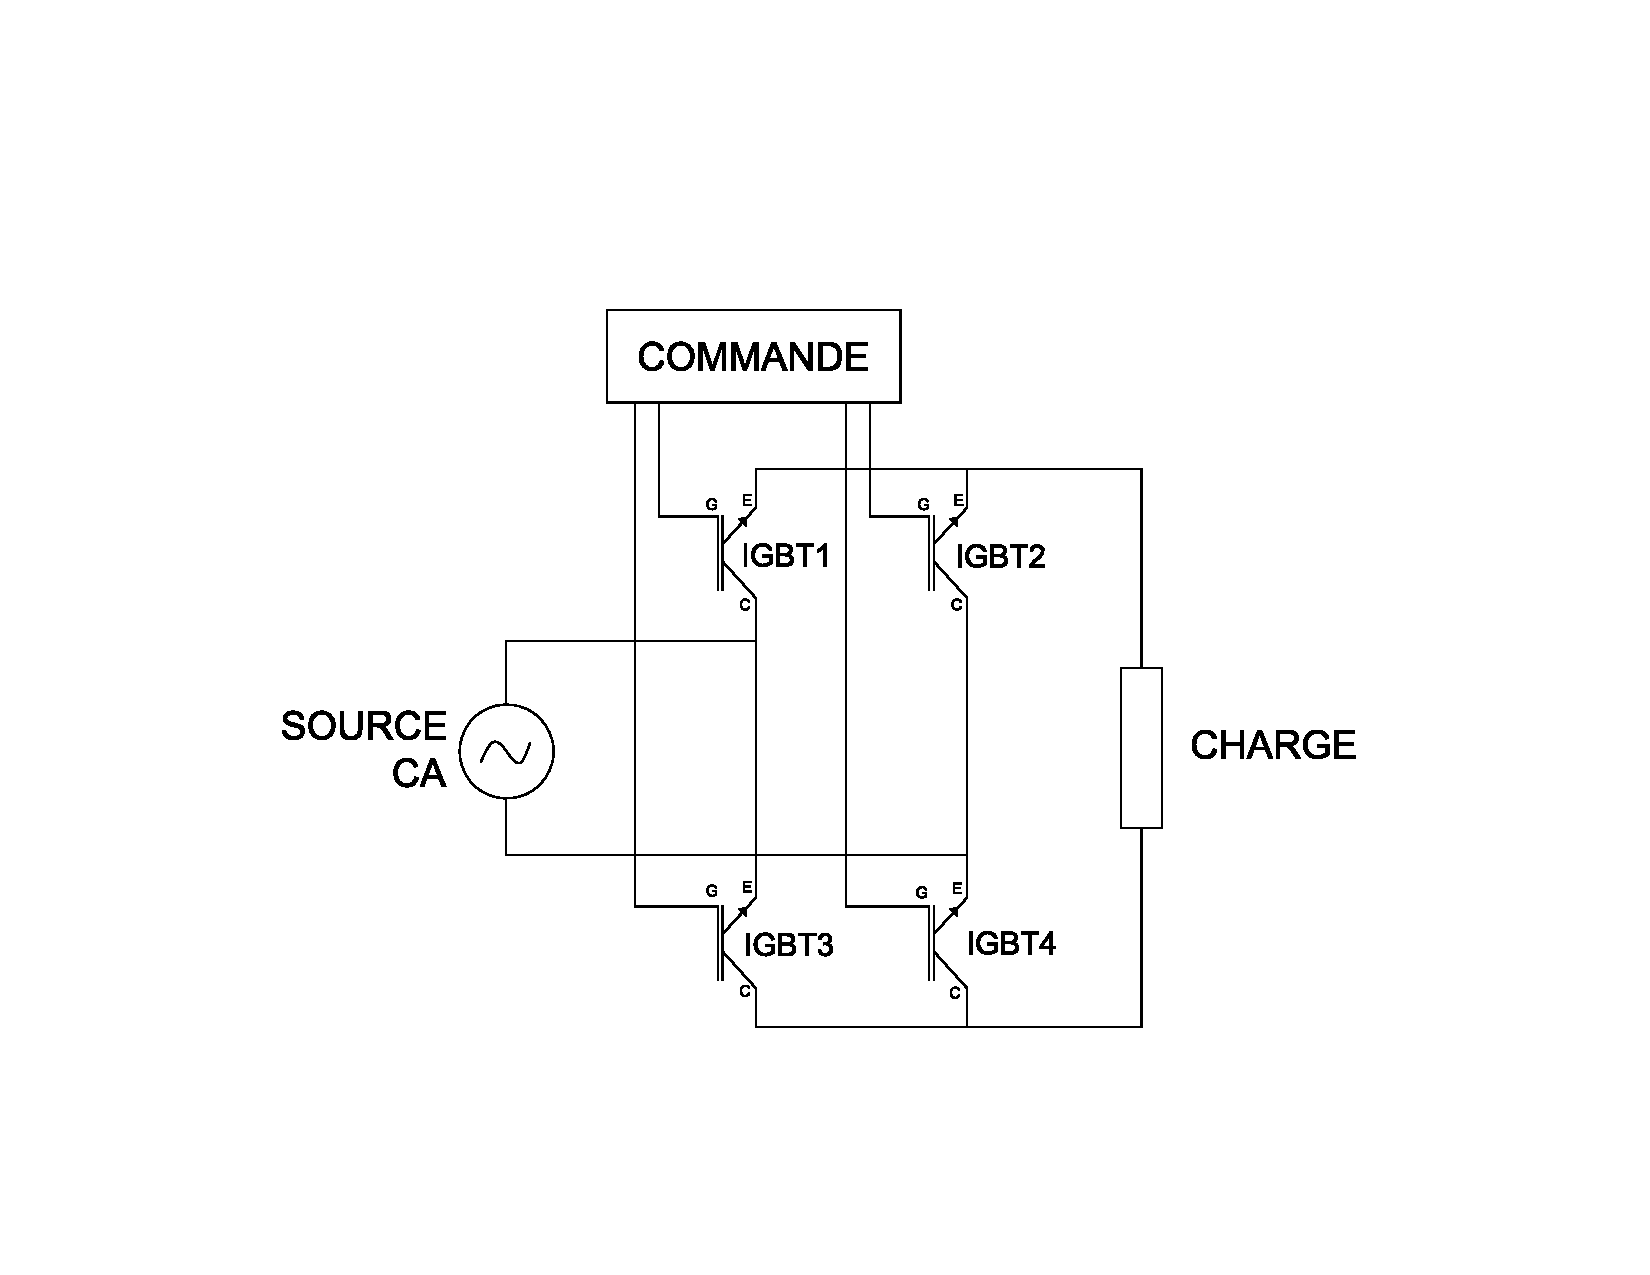
\includegraphics[width=0.7\textwidth]{Circuit/RedresseurMonophaseDoubleAlternanceIGBT}
    \caption{Circuit redresseur monophasé double alternance avec IGBT et charge quelquonque}
    \label{fig:RedresseurMonophaseDoubleAlternanceIGBT}
  \end{center}   
\end{figure}

\paragraph{}
La présence de l'alternance négative redressée permet deux modes de conduction, soit le mode continu et le mode discontinu. Comme les équations du système en régime permanent sont différentes dans les deux modes, il est nécessaire d'effectuer la résolution pour les deux différents cas.

\subsection{Mode continu}
Le redresseur double alternange opère dans le mode continu lorsque le courant dans la charge ne retombe jamais à zero. Ainsi, il est nécessaire d'adapter l'équation \ref{eq:solutionRLSimple} trouvée dans la section précédente. Nous savons que le courant dans la charge RL une fois l'inductance chargée est donné par :

\begin{eqnarray}
\label{eq:RedresseurMonophaseDoubleAlternanceContinu1}
i(t) &=& C_1\mbox{e}^{\frac{-t}{\tau}} + \frac{E_m\sin{(\omega_0 t - \phi})}{|Z|}
\end{eqnarray}

Où:
\begin{eqnarray}
C_1 &=& \left( I_1 - \frac{E_m\sin{(\omega_0 t + \phi})}{|Z|}\right)\mbox{e}^{\left(\frac{R}{L}\right)\left(\frac{\pi}{\omega_0}\right)}
\end{eqnarray}

En appliquant la condition $I_L(\omega_0 t = 0)=I_L(\omega_0 t=\pi)=I_1$ dans l'équation \ref{eq:RedresseurMonophaseDoubleAlternanceContinu1}, nous trouvons que :
\begin{equation}
\label{eq:RedresseurMonophaseDoubleAlternanceContinu2}
	I_1 = \frac{E_m\sin{(\phi)}}{|Z|}  \frac{1 + \mbox{e}^{\frac{-1}{\tau}}}{1 - \mbox{e}^{\frac{-1}{\tau}}}
\end{equation}

Finalement en allant remplacer $I_1$ dans l'équation \ref{eq:RedresseurMonophaseDoubleAlternanceContinu1} par l'équation \ref{eq:RedresseurMonophaseDoubleAlternanceContinu2}, nous trouvons que le courant dans la charge pour chaque demi-période une fois l'inductance chargée est :

\begin{equation}
	i(t) = \frac{E_m}{|Z|}\left[\sin{(\omega_0 t - \phi)} + \frac{2\sin(\phi) \mbox{e}^{\frac{-t}{\tau}}}{1-\mbox{e}^{\left(\frac{R}{L}\right)\left(\frac{\pi}{\omega_0}\right)}} \right] 
\end{equation}

\subsection{Mode discontinu}
Le redresseur double alternange opère dans le mode continu lorsque le courant dans la charge ne retombe jamais à zero. Ainsi, il est nécessaire d'adapter l'équation \ref{eq:solutionRLSimple} trouvée dans la section précédente. Nous savons que le courant dans la charge RL une fois l'inductance chargée est donné par :

\begin{eqnarray}
\label{eq:RedresseurMonophaseDoubleAlternanceContinu1}
i(t) &=& C_1\mbox{e}^{\frac{-t}{\tau}} + \frac{E_m\sin{(\omega_0 t - \phi})}{|Z|}
\end{eqnarray}

Où:
\begin{eqnarray}
C_1 &=& \left( I_1 - \frac{E_m\sin{(\omega_0 t + \phi})}{|Z|}\right)\mbox{e}^{\left(\frac{R}{L}\right)\left(\frac{\pi}{\omega_0}\right)}
\end{eqnarray}

En appliquant la condition $I_L(\omega_0 t = 0)=I_L(\omega_0 t=\pi)=I_1$ dans l'équation \ref{eq:RedresseurMonophaseDoubleAlternanceContinu1}, nous trouvons que :
\begin{equation}
\label{eq:RedresseurMonophaseDoubleAlternanceContinu2}
	I_1 = \frac{E_m\sin{(\phi)}}{|Z|}  \frac{1 + \mbox{e}^{\frac{-1}{\tau}}}{1 - \mbox{e}^{\frac{-1}{\tau}}}
\end{equation}

Finalement en allant remplacer $I_1$ dans l'équation \ref{eq:RedresseurMonophaseDoubleAlternanceContinu1} par l'équation \ref{eq:RedresseurMonophaseDoubleAlternanceContinu2}, nous trouvons que le courant dans la charge pour chaque demi-période une fois l'inductance chargée est :

\begin{equation}
	i(t) = \frac{E_m}{|Z|}\left[\sin{(\omega_0 t - \phi)} + \frac{2\sin(\phi) \mbox{e}^{\frac{-t}{\tau}}}{1-\mbox{e}^{\left(\frac{R}{L}\right)\left(\frac{\pi}{\omega_0}\right)}} \right] 
\end{equation}